\chapter*{Introduzione}
\addcontentsline{toc}{chapter}{Introduzione}

L'Internet delle cose è un termine descrittivo per riassumere una visione di
un futuro prossimo nel quale, sempre più dispositivi, riescano ad intercambiare
informazione senza l'ausilio umano. "IoT verrà utilizzato" In questa visione di 
un futuro non troppo lontano, termini quali, inteligent system transport, 
smart home automation, precision agriculture\cite{PAgricolture}, industrial 
automation, ecc.

Il mercato di questi \emph{smart devices } è
in rapida crescita con una stima di 8,3 miliardi di dispositivi connessi nel
anno 2017, e di circa 20 miliardi per l'anno 2020 \cite{gartner2016}. Andando ad
creare un impatto economico compreso tra i 2.7 e i 14 trilioni di dollari. I
mercati principali saranno quelli del healt care con un introito compreso tra i
$1.1$ e i $2.5$ trilioni di dollari e il settore industriale con $2.3$ a $11.6$
trilioni di dollari.

\begin{figure}[h]
\centering 
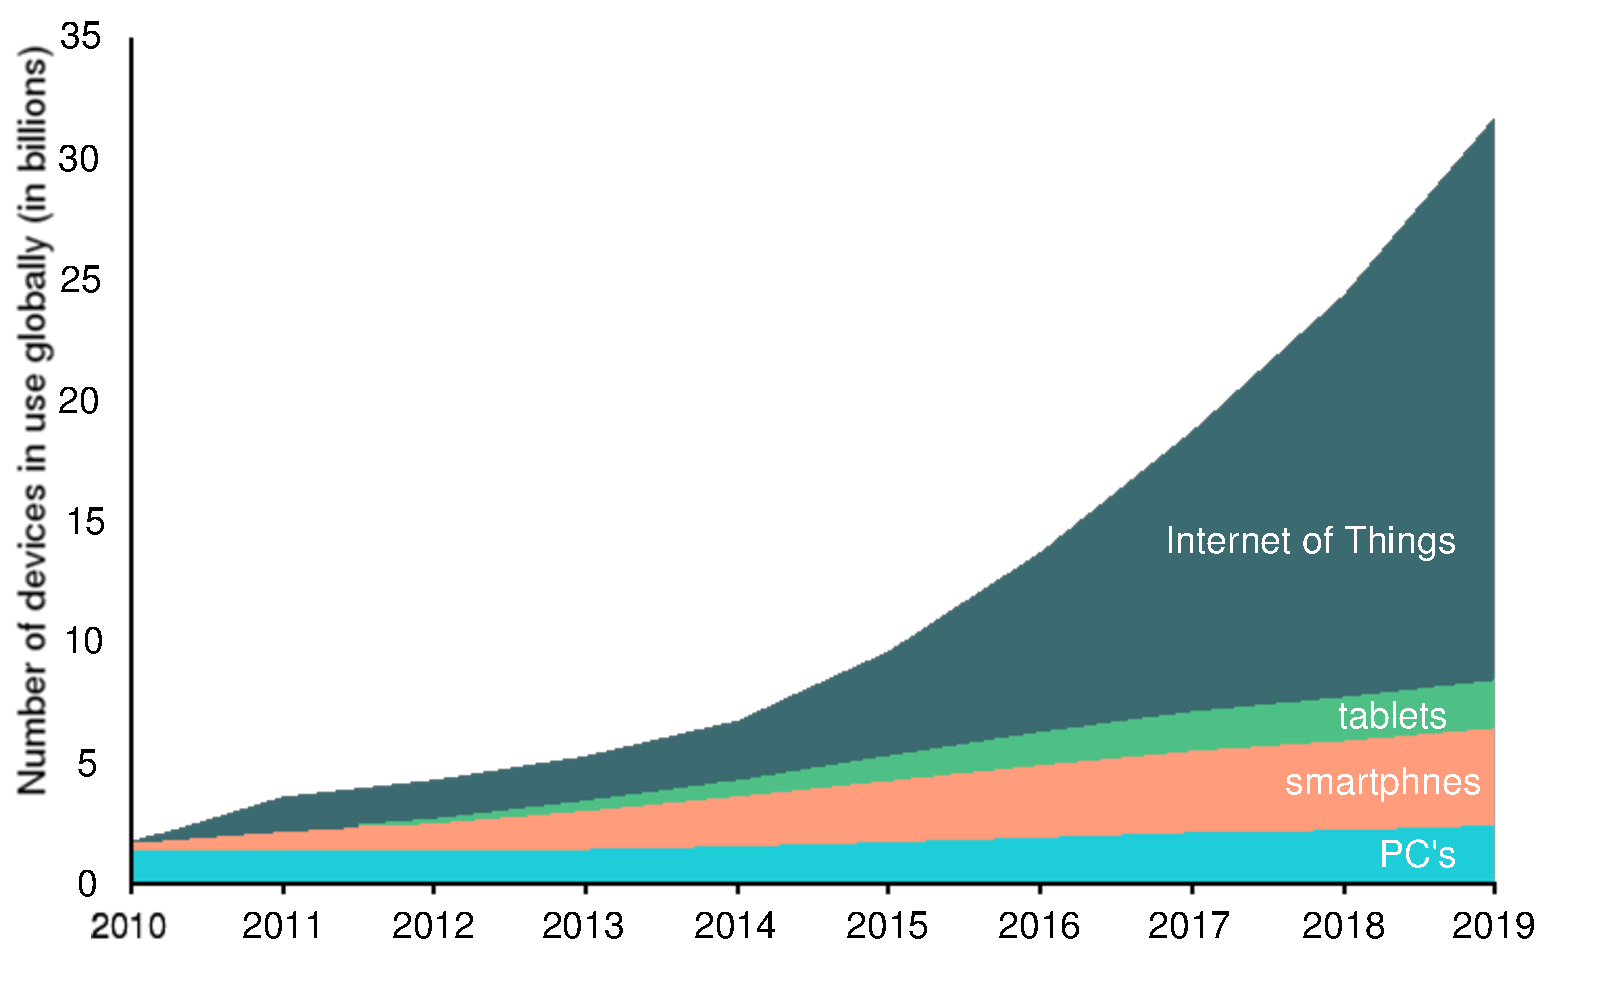
\includegraphics[width=10cm]{iot_devices}
\caption{Numero di dispositivi per anno}
\end{figure}

Questa rapida crescita ha portato alla ricerca è sviluppo di nuove soluzioni 
tecnologiche per supportare il carico di dispositivi simultaneamente connessi 
alla rete, senza avere un degrado evidente delle performance.
Per non alterare il \emph{QoS} Quality of Service della rete ed garantire costi
non elevati tecnologie come \emph{LPWAN} sono state ideate. I punti chiave per
garantire tutto ciò sono
\begin{itemize}
\item \textbf{Scalabilità}: Dato l'elevato numero di devices connessi, scenari
urbani ed industriali, la network tecnologi alla base dovrà essere estremamente
adattabile, in maniera dinamica, al carico di dispositivi connessi.
\item \textbf{Costo unitario}: Il costo del singolo modulo, dovrà essere basso
per garantire la più ampia fetta di mercato.
\item \textbf{Durata della batteria}: La maggior parte dei dispositivi sarà
alimentata tramite batteria, e la durata media e stimata di anni. 
\item \textbf{Costo computazionale}: La modulazione alla base di queste nuove
tipologie di rete, dovrà essere concepita in modo da non avere un costo
computazionale elevato.
\item \textbf{Distanza}: Un altro punto fondamentale è la possibilità di avere
comunicazioni a lunga distanza.
\end{itemize}

La rete di tipo \emph{LPWAN} è in grado di supportare tutti questi aspetti, le
principali tecnologie che già supportano questo tipo di rete son SigFox\tm,
LoRaWAN\tm, NB-IoT\tm e Weightless\tm. 

\begin{figure}[h]
\centering 
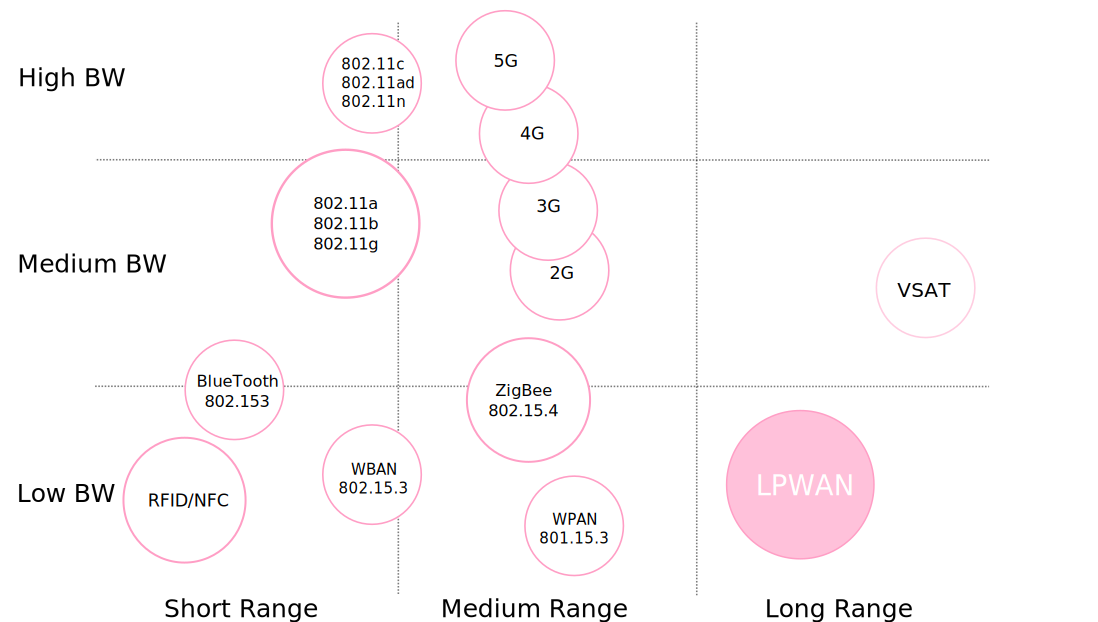
\includegraphics[width=16cm]{network_comp}
\caption{Comparazione tipologia di reti}
\end{figure}

Con questa tesi si è voluto studiare i casi applicativi della tecnologia Lora\tm
nel abito della agricoltura di precisione, utilizzando il framework open-source
Kura\tm messo a disposizione da Eurotech\tm, andando a creare un applicativo
OSGI\reg installabile nel framework. 
\begin{figure}[h]
\centering 
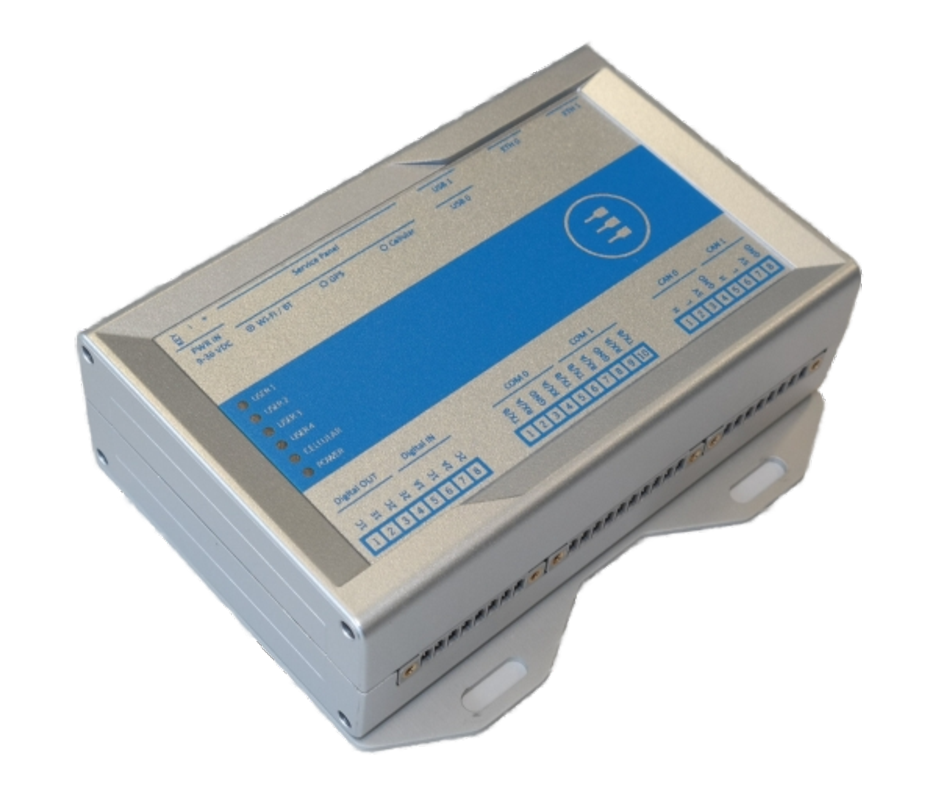
\includegraphics[width=10cm]{Reliagate_10_11}
\caption{Comparazione tipologia di reti}
\end{figure}

